\documentclass{iopconfser}

\usepackage{siunitx}
\usepackage{color}
\usepackage{mathtools}
\usepackage[normalem]{ulem}
\usepackage{adjustbox}
\usepackage{array}
\usepackage{booktabs}
\usepackage{multirow}
\usepackage{amsmath}
\usepackage{url}
\usepackage{natbib}

\newcommand{\todo}[1]{{\color{red}[TODO: "#1'']}}
\newcommand{\remove}[1]{ {\color{blue} \sout{#1}}}
\newcommand{\inblue}[1]{{\color{blue}#1}}
\newcommand{\inred}[1]{{\color{red}#1}}
\newcommand{\ingreen}[1]{{\color{green}#1}}
\newcommand{\soutred}[1]{{\color{red}\sout{#1}}}

\begin{document}

\title{WOFRY: a package for partially coherent beamline simulations in fourth-generation storage rings}

\author{Manuel Sanchez del Rio$^{1}$, Juan Reyes-Herrera$^{1}$, Rafael Celestre$^{2}$ and Luca Rebuffi$^{3}$}

\affil{$^1$European Synchrotron Radiation Facility, 71 Avenue des Martyrs, 38000 Grenoble, France}
\affil{$^2$Synchrotron SOLEIL, L'Orme des Merisiers Départementale 128, 91190 Saint-Aubin, France}
\affil{$^3$Argonne National Laboratory, 9700 South Cass Avenue, Lemont, Illinois 60439,, USA}

\email{srio@esrf.eu}


% -----------------------------------------------------------------
% -----------------------------------------------------------------
\begin{abstract}
We used a new software tool to perform coherent mode decomposition of the undulator radiation in 1D.  
\end{abstract}


     %-------------------------------------------------------------------------
     % The main body of the paper
     %-------------------------------------------------------------------------
     % Now enter the text of the document in multiple \section's, \subsection's
     % and \subsubsection's as required.

% -----------------------------------------------------------------
% -----------------------------------------------------------------
\section{Introduction}


xxx


% -----------------------------------------------------------------
% -----------------------------------------------------------------
\section{Modelling Sources}

A wavefront simulation consists of the creation of a wavefront with some characteristics (geometry, wavelength), its propagation in free space and its modification by the optical elements (slits, mirrors, etc). We restrict the description here to a 1D model in the ($x,y$) plane, with $y$ as the propagation direction (optical axis) and $x$ as the direction transverse to the beam propagation to analyze (usually the of horizontal or vertical plane). The wavefront is represented by the electric field of a monochromatic component (angular frequency $\omega$, wavelength $\lambda$, wavenumber $k = 2 \pi / \lambda$ or photon energy $W$) at a position $y=0$ along the propagation direction. This electric field or electric disturbance is a complex scalar $E(x;y=0,\omega)$ or, in case of polarized beams, two complex scalars, one for $\sigma$ and the other for $\pi$ polarization. The wavefront intensity is the square of the modulus of the amplitude: $I=|A \exp{(i\phi)}|^2=A^2$. 


% -----------------------------------------------------------------
\subsection{Simple waves: plane, spherical and Gaussian}

The simplest wavefront is a plane wave, with constant complex amplitude for any $x$ coordinate: 
\begin{equation}
   E(x;y=0,\omega)=E_0=A_0 e^{i \phi_0},
\end{equation}
where $E_0$ is a complex value that can be expressed in its constant real amplitude $A_0$ and a constant phase $\phi_0$. A plane wave is infinite along the $x$ direction. However, when representing a wavefront spatially, in simulation, the electric field has to be sampled over an array of discrete values of complex amplitude, and they are necessarily defined over a finite $x$ interval. 

A spherical wave (strictly speaking a circular wave in 1D, but we keep the terminology used in 2D) emanates from a fixed point and has a constant complex amplitude over a sphere of a given radius $R$. Obviously it cannot be represented at the source point ($y=0$, center of the sphere) and our wavefront must be sampled at a given distance $y=R$ and over a line perpendicular to the radius and tangent to the sphere. At $x=0$ (a point in the sphere) the field has a constant value equal to the value at the surface. But at a $x{\ne}0$, over a range of $x$-values $x{\ll}R$ (i.e. for small numerical apertures, NA) the distance from $x$ to the sphere parallel to the $y$ direction gives an optical path that modifies the phase by $k ~\Delta x$. It is easy to deduce that the wavefront in the line tangent to the sphere has the expression
\begin{equation}
\label{eq:sphericalWave}
    E(x;y=R,\omega)  = E_0 e^{i k x^2 / (2 R)}.
\end{equation}

% possible figure: 
% https://slideplayer.com/slide/730247/2/images/10/Spherical+wave+propagation.jpg

A Gaussian beam at the source position $y$=0 has constant phase and intensity following a Gaussian distribution with standard deviation $\sigma_I$, thus the electric disturbance is: 
\begin{equation}
\label{eq:gaussianSource}
    E(x;y=0,\omega) = E_0 e^{-x^2 / (4 \sigma_I^2)}
\end{equation}

% -----------------------------------------------------------------
\subsection{A simplified model for the undulator source}
\label{sec:undulator}

A single electron (or filament beam) traveling in an undulator with pure sinusoidal magnetic field in one direction will produce a complicated wavefront with geometry that varies as a function of the photon frequency (see, e.g., Ref.~\cite{elleaume}). At the resonance energy the angular emission in the far field can be approximated by a Gaussian function of width \cite{elleaume}
\begin{equation}
\label{eq:undulatorDivergence}
    \sigma'_u \approx\sqrt{\frac{\lambda}{2 L}},
\end{equation}
with wavelength of the photons at the undulator resonance, $\lambda$, and undulator length, $L$. At the source point, the size of the source can also be approximated by a Gaussian of width
\begin{equation}
\label{eq:undulatorSize}
    \sigma_u \approx\sqrt{\frac{\lambda L}{2 \pi^2}} = \frac{\lambda}{2 \pi} \frac{1}{\sigma'}.
\end{equation}

A  simplification of the undulator radiation in the far field consists in a spherical wave (Eq.\ref{eq:sphericalWave}) with origin in the undulator center modulated with an amplitude that follows the Gaussian in Eq.~\ref{eq:undulatorDivergence}, therefore
\begin{equation}
    \label{eq:undulatorBySphericalWave}
    E(x;y=y_0,\lambda) = E_0 e^{i k x^2 / (2 y_0)} e^{-x^2/(4 \sigma'_u{}^2 y_0^2)}.
\end{equation}

A second way to simulate the undulator is considering a Gaussian source as defined in Eq.~\ref{eq:gaussianSource} with $\sigma_I=\sigma_u$. Note that propagating this approximation of the undulator as a Gaussian source to a screen at $y=y_0$ does not reproduce the result in Eq.~\ref{eq:undulatorBySphericalWave} because Gaussian propagation implies a product of sigmas (emittance) of $\lambda / (4 \pi)$ whereas for undulator radiation the emittance is approximately $\lambda / (2 \pi)$ (Eq.~\ref{eq:undulatorSize}). For practical purposes, the Gaussian source approximation can be used for optical systems accepting a high NA, whereas for systems of small NA, as used in this paper, the spherical wave approximations may be preferred.

% -----------------------------------------------------------------
\subsection{Partial coherence modeling the undulator beam using coherent mode decomposition}

For the calculations presented in this paper we have developed a new tool for dealing with partially coherence beams produced by undulators in low-emittance storage rings. For that, we developed a 1D model of the coherent mode decomposition previously developed in 2D \cite{glass2017}. The motivation for developing these new tools is to perform quick calculations (e.g., being able to perform parametric calculations in a laptop) with high accuracy in the simulation of the source and beam propagation. We believe that the separation of the real 2D wavefront in two separated 1D wavefronts is well justified for most synchrotron beamlines, where the cross-talk between these two directions is small. 
The tools developed here are included in the OASYS toolbox \cite{codeOASYS}, available in the WOFRY add-on \cite{XX}. These tools are completely scriptable so they can be used from the OASYS interface, which also creates scripts that can be a posteriori modified for batch runs. 


The electrons in an storage ring are statistically distributed, following (in good approximation) a Gaussian distribution in a 6-dimensional space (three spatial coordinates, two angles to define direction, and the electron energy). Many electrons therefore contribute to photon beam radiation, each one creating a wavefront. The consequence is that the overall radiation cannot be described deterministically which implies that statistical methods are needed, like for describing the electron beam. This is the origin of partial coherence of the synchrotron emission. As stated before, in an ideal storage ring of zero emittance, the electrons follow a filament beam so the emission is fully coherent. As soon as  electron emittance increases, the electrons contributing to the radiation start to have different initial conditions (in the 6-dimensional space) and the overall emission cannot be describe by a single wavefront, but by statistically distributed wavefronts, described by partial coherent optics.

Under some approximations the radiation is 'wide sense stationary' \cite{mandel_wolf}. These conditions are satisfied for light emitted by storage rings (but not for XFELs) \cite{geloni2008}, and can be summarized in
i) the electron bunch length is long enough,
ii) radiation is monochromatized 'not too much' (like by standard monochromators), and 
iii) the radiation frequency is large enough.
It is in this case all the coherent properties of the radiation can be described using the 'cross spectral density' (CSD), a complex function that measures the correlation of the electric field in two different spatial points at a given radiation frequency. It can be mapped in a $(x,y)$ plane at a third coordinate $z$. At that plane, the CSD depends on 5 variables: 

\begin{equation}
W_{2D}(x_1,y_1,x_2,y_2;\omega) = <E^*(x_1,y_1;\omega) E(x_2,y_2;\omega)>
\label{eq:CSD_1D}
\end{equation}

In the following, we suppose that the CSD is separable in its 1D horizontal $x$ and vertical $y$ coordinates, therefore the $W_{2D}$ becomes a product of two CSD functions $W$ of two variables for a given photon frequency $\omega$:

\begin{equation}
W_{2D}(x_1,y_1,x_2,y_2;\omega) = W(x_1,x_2;\omega) W(y_1,y_2;\omega).
\label{eq:CSD_2D}
\end{equation}
Each $W$ function is treated separately in a similar way affecting the $x$ (horizontal) and $y$ (vertical) coordinate.

From the cross spectral density one can calculate the 'spectral density' (usually simply called 'intensity') $I(x;\omega)=W(x,x,\omega)$, and also the complex degree of (transverse) coherence: 
\begin{equation}
\mu(x_1,x_2;\omega) = \frac{W(x_1,x_2;\omega)}{\sqrt{I(x_1;\omega)}\sqrt{I(x_2;\omega)}}
\label{eq:DTC}
\end{equation}
The modulus of the complex degree of coherence is one for a completely coherent beam and zero for an incoherent beam. 

An important result in partial coherence optics permits to describe the radiation as an infinite sum of independent coherent modes (in the sense of orthonormality) :

\begin{equation}
W(x_1,x_2;\omega) = \sum_{n=0}^{\infty} \lambda_n(\omega) \Phi_n^*(x_1;\omega) \Phi_n(x_2;\omega) 
\label{eq:CMD}
\end{equation}
where $\lambda_n$ (eigenvalues) are the intensity weights and the $\Phi_n$ are the coherent modes (eigenfunctions). 
Some important characteristics of this coherent mode decomposition are: i) the modes are orthonormal (in the integral sense), ii) the modes maximize the spectral density, the first mode is more intense than the second, and so on, meaning that the truncated expansion is optimal, and iii) there is complete coherence if and only if there is only a single mode. If one can truncate the infinite series to a limited number of modes $N$ which contain a good percentage of the spectral density, the numerical storage of the $N$ modes that depend on two spatial variables is usually more economic than the storage of the cross spectral density $W$ that depends on four variables. 
The eigenvalues $\lambda_n$ are a measure of the intensity. Indeed, one can define the occupation $\eta$ of the i-th mode as the ratio of its intensity to the total intensity: 

\begin{equation}
\eta_i(\omega) = \frac{\lambda_i(\omega)}{\sum_{n=0}^{\infty} \lambda_n(\omega)}
\end{equation}

From these arguments, it is now natural to rigorously define Coherent Fraction ($CF$) as the occupation of the first coherent mode: $CF=\eta_0$.

The eigenvalues and the coherent modes are obtained by performing the Coherent mode decomposition (CMD). They are solution of the homogeneous Fredholm integral equation of second kind \cite{glass2017}. This is an eigenvalue problem. The numerical solution is obtained from the diagonalization of the CSD, which is a multivariate tensor when sampled at the point coordinates. This diagonalization problem is solved in 2D (i.e., $W_{2D}$ is a function of 4 variables) using complex numerical algorithms implemented in COMSYL. Fortunately, in 1D, the CSD is a function of two variables, represented in a matrix that can be easily diagonalized using standard tools availables in python-numpy. The numerical calculation of $W(x_1,x_2)$ uses Kim's convolution theorem \cite{kim1986b} as described in \cite{glass2017}. It includes two ingredients: i) the statistical parameters of the electron beam at the undulator center (sizes and divergences), and ii) the intensity distribution of the undulator emission at the undulator center. The undulator emission is calculated in a plane far enough from the undulator using classical electrodynamics \cite{jackson} (as implemented in the pySRU python library \cite{pySRU}), and then backpropagated (using a Fresnel propagator) to the center of the undulator. 

It is important to calculate the real emission of the undulator which is very different than a Gaussian. However, the (inadequate) use of a Gaussian approximation for the undulator radiation is often found in literature, e.g.  \cite{coisson1997}. In this case the Kim convolution predicts a CSD that is identical to the Gaussian Shell-method (GSM). Parameters of the undulator approximated by a GSM can be calculating by matching the coherent as explained in Appendix \ref{appendix:matchCF}). There is another argument in favour of using non-approximated coherent modes: small differences in a mode in terms of shape (even maintaining the same FWHM) may give to completely different results after propagation. Moreover, the GSM modes are real functions (constant phase) whereas the modes from CMD of undulator sources are complex functions (with a non-constant phase).

The interest of the coherent mode decomposition method is twofold: the possibility to propagate a partial coherent beam along the beamline by just propagating a few modes (less modes for a more coherent beam) which behave like coherent wavefronts, and the use of the coherent fraction (a scalar parameter) as a accurate well-defined measure of how coherent is the beam at any position of the beamline.


% -----------------------------------------------------------------
% -----------------------------------------------------------------
\section{Free space propagators}
\label{sec:propagators}


For simulating the beamline, the wavefront at the source has to be created using the methods in section  \ref{sec:sources}, and then the optical elements modify sequentially the wavefront using the algorithms described in section \ref{sec:elements}.  But the wavefront evolves when transported in free space from element to element. We use here two propagators. 

% -----------------------------------------------------------------
\subsection{Direct implementation of integral Rayleigh-Sommerfeld propagator}
\label{sec:integralPropagator}

The Rayleigh-Sommerfeld propagator for small-angle approximation expresses the electric field at a spatial point $\vec{r}'$ as an integral of the electric field at a spatial point $\vec{r}$ \cite{goodmanfourier}
\begin{equation}\label{eq:RSpropagator}
E(\vec{r}') =  \frac{k}{2 \pi i} \int \frac{E(\vec{r})}{|\vec{r}'-\vec{r}|} e^{ i k |\vec{r}' - \vec{r}|  }  d\Sigma,
\end{equation}
where the integral is made over the domain of the source (the surface $\Sigma$). 
This propagator can be applied to numerical discrete 1D wavefronts, and the integral reduces to a sum
\begin{equation}\label{eq:discreteRSpropagator}
E(x_1,y_1) \approx \frac{k}{2 \pi i \Delta y}  \sum_{i=0}^{N-1}  E(x_{0,i},y_{0,i}) e^{i k \sqrt{(x_1 - x_{0,i})^2 + (y_1 - y_{0,i})^2} }  \Delta x_0,
\end{equation}
where $\Delta y$ is the mean value of the denominator in the integral in Eq.~\ref{eq:RSpropagator}.
Note that one sum over the $N$ points of the sampled incident wavefront has to be done for each coordinate at the transported wavefront, thus the number of operations is of the order $N^2$. This simple propagator gives flexibility to define different gridding and limits permitting the adjustment of the spatial domain or window and spatial resolution when working with converging or divergent wavefronts. Moreover, the propagated wavefront can be computed in a plane (or line) non parallel to the incident one, a feature that is exploited in sections~\ref{sec:grazingReflector} and \ref{sec:grating}. 


% -----------------------------------------------------------------
\subsection{Fresnel propagator using FFT: The zoom propagator}
\label{sec:zoomPropagator}


The Fresnel propagator is obtained by making a Taylor expansion of the quadratic phase in Eq.~\ref{eq:RSpropagator}: 
\begin{equation}\label{eq:fresnelPropagator}
E(x;y_1) =  \frac{e^{i k (y_1-y_0)}}{\sqrt{i \lambda (y_1-y_0)}} \int E(x';y_0) e^{ \frac{i k}{2 (y_1-y_0)}  (x-x')^2  }  dx'.
\end{equation}

The Fresnel integral propagator can be seen as convolution of the wavefield with a Gaussian kernel. One can write Eq. \ref{eq:fresnelPropagator} in convolution form, involving \inblue{a Fourier transform $\mathcal{F}$ and an inverse Fourier transform $\mathcal{F}^{-1}$}\cite{goodmanfourier}:
\begin{equation}\label{eq:fft}
E(x; y_1) = \inblue{P^G} \mathcal{F}^{-1}\Big\{ \mathcal{F}\{E\} K \Big\},
\end{equation} 
where \inblue{$E$ is the electric perturbance at $y_0$ $E(x;y_0)$, $P^G=e^{i k (y_1-y_0)}$ is a global phase and $K=e^{-i \pi \lambda (y_1-y_0) u^2}$ is the Gaussian Kernel } that comes from the inverse Fourier Transform of the exponential inside the integral in Eq.~\ref{eq:fresnelPropagator}, being $u$, the conjugated variable of $x$.
The real benefit of using this scheme comes from the use of Fast Fourier Transforms, that reduce the number of operations from $N^2$ to $N \log_2 N$. Its use is essential when doing simulations in 2D, because the direct calculation of the integral lead to $N^4$ operations at the limit of calculation power of usual laptop computers. However, the FFT implementation requires that the gridding and spatial domain of the incident and transported wavefronts must be equal. This is a problem when a wavefront is propagated to a focal point: the gridding of the incident wavefront used at the image provides a poor resolution because most of the intensity is concentrated in a very few pixels. A clever solution to this problem is presented by J.D. Schmidt \cite{schmidt} that makes possible to calculate the propagated field in a ``zoomed'' window, thus permitting optimizing the wavefront sampling in cases for propagating highly convergent or divergent wavefronts. The problem reduces to a convolution problem of the unpropagated field field $E(x;y_0)$ affected by a phase $P$ with a kernel $K$, and the result affected by a global phase $P^G$: 
\begin{equation}
E(x; y_1) = P^G \mathcal{F}^{-1} \Big\{ \mathcal{F} \big\{ E~~P \big\} K \Big\},
\end{equation}
where
\begin{equation}
P^G =  \frac { e^{ik(y_1-y_0) }}{\sqrt{m_x} }e^{i \frac{k}{2 (y_1-y_0)} \frac{m_x - 1}{m_x}x_2^2},
\end{equation}
\begin{equation}
P = e^{i \frac{k}{2(y_1-y_0)} (1-m_x)x_1^2 },
\end{equation}
\begin{equation}
K = e^{-i \pi \lambda (y_1-y_0) \frac{u^2}{m_x} }.
\end{equation}
The term $m_x$ is the magnification (zoom) factor. 
Note that setting unity magnification $m_x=1$, one obtains the standard Fresnel propagator (Eq.~\ref{eq:fft}).

% -----------------------------------------------------------------
% -----------------------------------------------------------------
\section{Modeling beamline elements}
\label{sec:elements}

In cases where the distance between elements is significantly greater than the mirror sizes, the optical elements can be approximated as thin elements (zero thickness along the $y$ axis), and their effect can be encapsulated in a complex transmission amplitude,
\begin{equation}
    \label{eq:thinelement}
    R(x;\omega)=r(x;\omega) e^{i \rho(x,\omega)}.
\end{equation}
Therefore, the wavefield after an optical element placed at position $y=y_0$ will be the wavefield at $y_0$, just before the interaction, multiplied by the complex transmission:
\begin{equation}
    E'(x;y=y_0,\omega) = E(x;y=y_0,\omega) R(x;\omega)
\end{equation}

% -----------------------------------------------------------------
\subsection{Apertures}

A generic aperture is a mask that transmits a part of the wavefront in a range $[x_{min},x_{max}]$ and absorbs the rest. It can be
\begin{equation}
R(x;\omega) =
\left\{
\begin{matrix}
A,  & \mbox{~~if~~} x_{min} \le x \le x_{max}
\\ 
1 - A, & \mbox{~~elsewhere}
\end{matrix}
\right.
\end{equation}
When the element is a slit, then $A=1$. If it is a beamstop, then $A=0$. In the following simulations we will use an aperture of finite length $a$ centered with the beam, therefore $x_{min}=-a/2$ and $x_{max}=a/2$.

A sometimes useful case is the ``Gaussian slit" where $A=\exp(-x^2/(2\sigma_a))$. \todo{check is Gaussian applies to amplitude or intensity (in that case is divided by 4 instead 2)} The aperture acts as a Gaussian appodization window. Although artificial, it is interesting to shape the beam with a Gaussian profile, which remains a Gaussian after propagation. Therefore, a Gaussian slit acting on a plane wavefront does not produce diffraction fringes. Several recipes are proposed to relate $\sigma_a$ with the slit aperture $a=x_{max}-x_{min}$. We found convenient to define $\sigma_a=\Delta a/2.355$ (see Appendix \ref{appendix:slit}).


% -----------------------------------------------------------------
\subsection{Mirrors}


\subsubsection{Ideal mirror}
\label{sec:idealReflector}

Let us consider a perfectly reflecting surface (no absorption) with a profile $h(w)$ with $h$ the elevation (height) and $w$ the linear coordinate in a reference frame attached to the reflector with origin in the reflector's center. A plane reflector has $h(w)=0$ and, for example, a circular mirror of radius $R$ has $h(w)=R-\sqrt{R^2 - w^2}$. The profile $h(w)$ can also match a deformation originated for instance by heat load or a mirror surface error (waviness).

If the reflector is set with an incident angle $\theta$, with the propagation axis $y$, the change of optical path is $\Delta y = 2 h(w) \sin \theta$, $w=x/\sin\theta$, with a consequent phase shift $\Delta \Phi = - k \Delta y $, therefore for the ideal reflector
\begin{equation}
\label{eq:idealReflector}
    R(x;\omega) = e^{-2 i k h(w) \sin \theta}.
\end{equation} 

This model of ideal reflector as a thin object  can be used for any reflecting shape (circular, ellipse, etc.) but the intrinsic aberrations are not correctly considered.  The main reason is the incidence angle $\theta$ is not constant along the mirror profile thus Eq.~\ref{eq:idealReflector} is not exact. A model for a ``grazing reflector" that solves this problem is presented in the next section \ref{sec:grazingReflector}.

A reflector of a finite size can be decomposed in two elements: the ideal reflector described here, followed (or preceded) by the aperture as described in \ref{sec:aperture}.

\subsubsection{Grazing incidence mirror}
\label{sec:grazingReflector}

The method used for the {\it ideal reflector} does not account for mirror aberrations and it is not exact when dealing with mirror errors because the optical path is approximated. These effects are more important for elements in grazing incidence, where the {\it thin object} approximation is not valid. A solution for that consists in using the propagator in Sec.~\ref{sec:integralPropagator} to propagate the incident wavefront until the points in the mirror surface $(w,h)$. Let be $p$ the distance from the wavefront $E_0(x,;y=0,\omega)$ to the center of the mirror placed at a grazing incidence $\theta$ with the optical axis. In the mirror reference frame, the wavefront coordinates are $(w_s, h_s) =(-p \cos \theta, p \sin \theta) + (x \sin \theta, x \cos \theta)$. It is straightforward to extend the integral propagator (Eq.~\ref{eq:discreteRSpropagator}) to calculate the propagated field at the surface points $(w,h)$ by summing over all points of the input wavefront. Once the electric perturbation at the mirror surface is known, another propagation is performed using the same principle, to the image plane placed at a distance $q$ from the mirror center.

% -----------------------------------------------------------------
\subsection{Gratings}
\label{sec:grating}

A grating produces a diffraction of the incident beam that is dependent on its wavelength. It is expressed by the grating equation:
\begin{equation}
    m \lambda g = \sin\alpha + \sin\beta,
\end{equation}
with $\alpha$ the incidence angle (measured with respect to the normal), $\beta$ the reflection angle, with opposite sign of $\alpha$ if it lies at the other side of the normal, $m$ the diffraction order (positive for inside reflection, i.e., $\alpha \ge |\beta|$),
%(note than in SHADOW is the contrary, inside orders are negative)
$\lambda$ is the photon wavelength, and $g$ is the grating groove density, which is a function of $w$ for VLS gratings: $g = g_0 + g_1 w + g_2 w^2 + ...$ with $g_0 = 1/d_0$ the lines per unit of length at the grating center ($d_0$ the distance between two grating lines).

The simulation of a grating using a thin object model (Eq.~\ref{eq:idealReflector}) is difficult because in addition to the geometric optical path it is necessary to account for the wavelength-dependent component. We use here an approach that is exact, except for accounting for the diffraction efficiency, which consisting of sampling the grating as a numeric mesh and apply the ``grazing reflector." 
This model also permits to study line spacing errors together with height errors of the substrate. It is important not to undersample the grating (e.g., we must include several points per period) and orientate the incident and image wavefronts with the correct angles $\alpha$ and $\beta$.

% -----------------------------------------------------------------
\subsection{Refractive systems}

\subsubsection{Ideal lens}
We can define an ideal lens as a focusing device that converts a plane wave into a spherical wave collapsing to the focus at a distance $f$ from the ideal lens position. Therefore
\begin{equation}
    R(x;\omega) = e^{-i k~x^2/(2 f)}.
\end{equation}

An ideal coupling of $N$ ideal lenses will present a focal length $f=(f_1^{-1}+f_2^{-1}+...+f_N^{-1})^{-1}$. 

\subsubsection{Thin object} A refractor made by a material with refraction index $n(\omega)=1-\delta(\omega)+i\beta(\omega)$ 
%($n$ depends the photon wavelength $\lambda$)
and thickness profile $z(x)$ adds a phase to the wavefront $-\lambda \delta(\omega) z(x)$ and reduce its amplitude by $\exp(-\mu z(x)/2)$, where $\mu=(4 \pi/\lambda) \delta(\omega)$ is the (intensity) attenuation coefficient and $\lambda$ the photon wavelength. These expressions can be applied to any transmission object of profile $x(z)$ assuming valid the thin object approximation. 

\subsubsection{Real lens} The changes induced by a real lens in the wavefront can be calculated using the thin object approximation discussed below, using the lens profile. Usually, a single lens has a parabolic profile $z=x^2/(4R)$ with $R$ the radius of the apex. A lens has two parabolic profiles (front and back) separated by a lens thickness $d$ and a flat profile outside the lens aperture $L$, therefore:
\begin{align}
    z(x) &= \frac{1}{2R} z^2 + d; & x < L/2\\ \nonumber
    z(x) &= \frac{1}{2R} (L/2)^2 + d; & x \ge L/2.
\end{align}

\subsubsection{CRLs and transfocators}
A Compound Refractive Lens is a pile of $N$ identical lenses. If we consider negligible the beam propagation in the inter-lens space, the effect of the $N$ lenses is identical of a single lens with profile $x_N(z)=N z(x)$. If one is interested in assessing the effect of the inter-lens space (e.g. for studying the adiabatic focusing)  the CRL must be calculates as $N$ independent lenses, applying the free-space propagator in between two consecutive lenses. For transfocators (a transfocator is a pile of CRLs) the same concepts apply: it is possible to compute the accumulated lens profile and use it as a single lens, or calculate lens by lens (or CRL by CRL) if the effect of inter-lens or inter-CRL spaces are to be taken into account.

\subsubsection{Lens errors}
The profile of a real lens $z(x)$ can be decomposed in the ideal parabolic profile (best fitted parabola) $z_P(x)$ plus a residual profile (errors) $z_{error}(x)$. One can then apply the thin object approximation with this profile. 

\subsubsection{Refractive corrector}
\label{sec:refractorCorrector}
One can imagine a refractive object to focus an arbitrary incoming wavefront to a given point placed at a distance $D$. In other words, this object would transform the incoming wavefront into a spherical (circular in 1D) wavefront collapsing to the focus. The profile of such refractive ``corrector"  can be calculated using the phase difference $\Delta\phi(x)=\phi_S(x)-\phi(x)$ where $\phi_S=k x^2 / (2 D_w)$ is the phase of the circular wave collapsing at $D_w$, $k$ is the wavenumber ($k=2\pi/\lambda$) and $\phi$ is the phase of the incoming wavefront. The corrective profile is $z(x)=-\Delta\phi/(k \delta(\omega))$.



% -----------------------------------------------------------------
% -----------------------------------------------------------------
\section{Simulations of the complete beamline}


% -----------------------------------------------------------------
\subsection{Example of an ESRF beamline}
xxx


% -----------------------------------------------------------------
\subsection{Example of an APS beamline}
xxx


% -----------------------------------------------------------------
% -----------------------------------------------------------------
\section{Discussion}

% -----------------------------------------------------------------
\subsection{Undulator coherent modes versus Gaussian-hermite modes}

xxx

% -----------------------------------------------------------------
\subsection{Coherent fraction out of resonance}

xxx

% -----------------------------------------------------------------
% -----------------------------------------------------------------
\section{Discuss grazing optics and surface errors}

% -----------------------------------------------------------------
% -----------------------------------------------------------------
\section{Summary and conclusions}
\label{sec:summary}

xxx


%%%%%%%%%%%%%%%%%%%%%%%%%%%%%%%%%%%%%%%%%%%%%%%%
%%%%%%%%%%%%%%%%%%%%%%%%%%%%%%%%%%%%%%%%%%%%%%%%
%%%%%%%%%%%%%%%%%%%%%%%%%%%%%%%%%%%%%%%%%%%%%%%%
% \appendix

% -----------------------------------------------------------------
% -----------------------------------------------------------------
\section{The Coherent Fraction predicted by the Gaussian Shell-model and its aplication to approximate undulator sources}
\label{appendix:matchCF}
The Gaussian Shell-model is a case for partial coherent beams well know in optics, as it models quite well the lasers beams, and it is analytic. It is a 1-dimensional where both the spectral density (intensity distribution) and the degree of transverse coherence between two points follow Gaussian distributions, described by standard deviations $\sigma_I$ and $\sigma_{\mu}$, respectively. The cross spectral density is
\begin{equation}
W(x_1,x_2,\omega) = A^2 e^{-(x_1^2+x_2^2)/(4 \sigma_I^2)} e^{-(x_2-x_1)^2/(2 \sigma_{\mu}^2)}
\label{GS_CSD}
\end{equation}
with $A$, $\sigma_I$ and $\sigma_{\mu}$ positive constants that depend on $\omega$.
This cross spectral density can be decomposed in coherent modes
\cite{Starikov82,mandel_wolf} 
\begin{equation}
W(x_1,x_2,\omega) = \sum_{n=0}^{\infty} \lambda_n(\omega) \Phi^*(x_1,\omega) \Phi(x_2,\omega). 
\label{CMD}
\end{equation}
The $\lambda_n$ (eigenvalues) are
\begin{align}
\lambda_0 &= A \sqrt{\pi/( a+b+c)}; \\ 
\lambda_n &= \lambda_0 q ^n,
\end{align}
with $a = (4 \sigma_I^2)^{-1}$, $ 
b = (2 \sigma_{\mu}^2)^{-1}$, $ 
c = (a^2 + 2 a b)^{1/2}$,
\begin{equation}
q = \frac{1}{1 + \beta^2/2 + \beta\sqrt{(\beta/2)^2+1}} 
\label{q}
\end{equation}
and $\beta=\sigma_{\mu}/\sigma_I$. 

The eigenfunctions are
\begin{equation}
\Phi_n(x) = \left( \frac{2c}{\pi} \right)^{1/4} \frac{1}{\sqrt{2^n n!}} H_n(x\sqrt{2c})e^{-cx^2}
\label{GSeigenvalues}
\end{equation}
with $H_n$ are the physicist's Hermite polynomials of order $n$. 

The occupation of coherent modes, or normalized eigenvalues is   
\begin{equation}
\eta_n = \frac{\lambda_n}{\sum_{i=0}^{\infty} \lambda_i} = q^n(1-q), 
\end{equation}
thus the coherent fraction is $CF=\eta_0=1-q$, and the cumulated occupancy
\begin{equation}
\ \sum_{i=0}^{n-1} \eta_i = 1-q^n. 
\end{equation}
From here one can calculate the number of modes needed to reach a cumulated occupancy $c_0$, which is $n=\ln(1-c_0)/\ln q$.

For representing the undulator radiation by a GSM, we need to obtain the $\sigma_I$ and $\sigma_\mu$ values. The intensity $\sigma_I$ matches the intensity distribution of the undulator source that is usually approximated as the convolution of the electron bunch size $\sigma_x$ with the radiation cross section $\sigma_u$. The other GSM value is $\sigma_\mu=\beta\sigma_I$, and $\beta$ is obtained via $q$ by matching the GSM coherence fraction $CF=1-q$ with the undulator coherence fraction approximated by
\begin{equation}
    CF_u = \frac{\sigma_u\sigma_{u'}}{\sqrt{\sigma_x^2+\sigma_u^2}\sqrt{\sigma_{x'}^2+\sigma_{u'}^2}}.
\end{equation}
Therefore, the GSM $\beta$ is obtained by $\beta=CF_u/\sqrt{1-CF_u}$,
and the radiation parameters are $\sigma_{u'}=\sqrt{\lambda/(2L)}$, $L$ the undulator length and $\sigma_u \sigma_{u'} \approx \lambda / (2 \pi)$.

% -----------------------------------------------------------------
% -----------------------------------------------------------------
\section{Validity of GSM for coherent mode decomposition of undulator radiation}
\label{appendix:validity}

We have calculated here the coherent mode decomposition for the U2 undulator (N=100, K=1.19) at the EBS storage ring. 

In a first step the coherent mode decomposition of the undulator radiation has been performed using a 1D model. The results are compared with the GSM approximation. Results for the horizontal direction are in (Fig.~\ref{fig:GSMvsUND-H}) in (Fig.~\ref{fig:GSMvsUND-V}) for the vertical one. As expected, these figures shows that the GASm is a good approximation for cases where the coherence fraction is small (the horizontal case) but the results are very different, in particular the eigenfunctions, in the case of high coherence (vertical direction in Fig.~\ref{fig:GSMvsUND-V}).


\begin{figure}
    \centering
    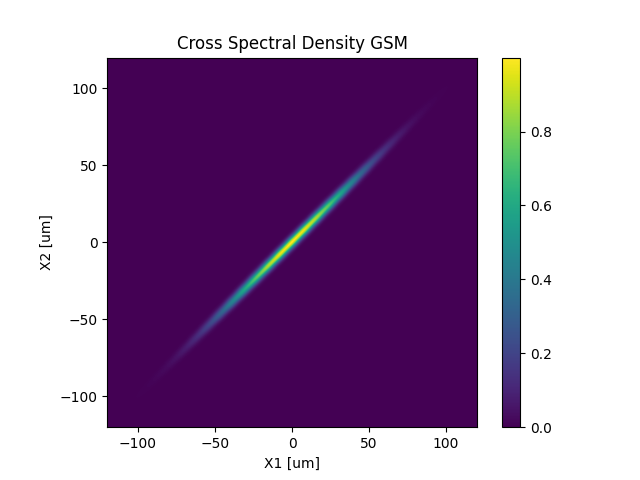
\includegraphics[width=0.49\textwidth]{figures/comparison_H_CSD_GSM.png}
    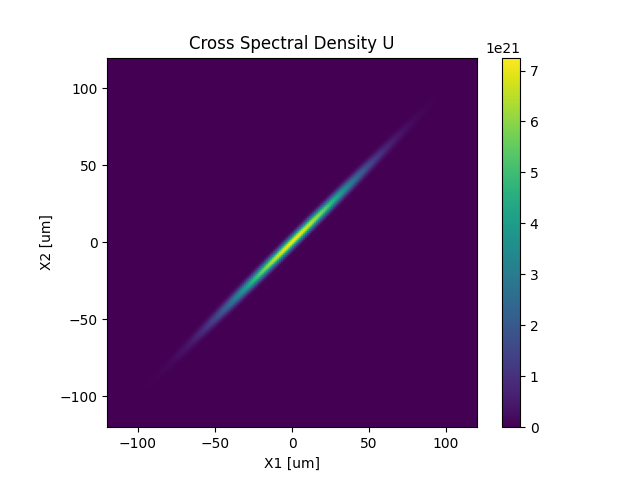
\includegraphics[width=0.49\textwidth]{figures/comparison_H_CSD_U.png}
    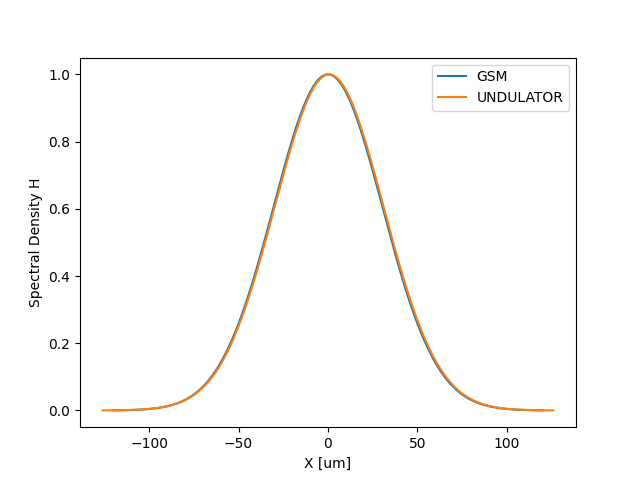
\includegraphics[width=0.59\textwidth]{figures/comparison_H_SD.png}
    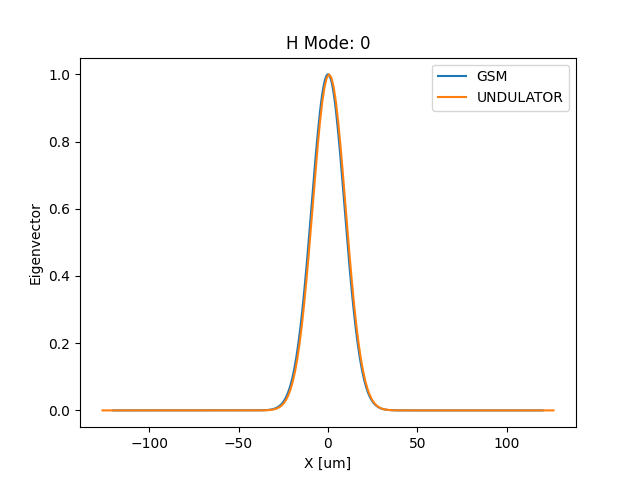
\includegraphics[width=0.49\textwidth]{figures/comparison_H_eigenvector0.png}
    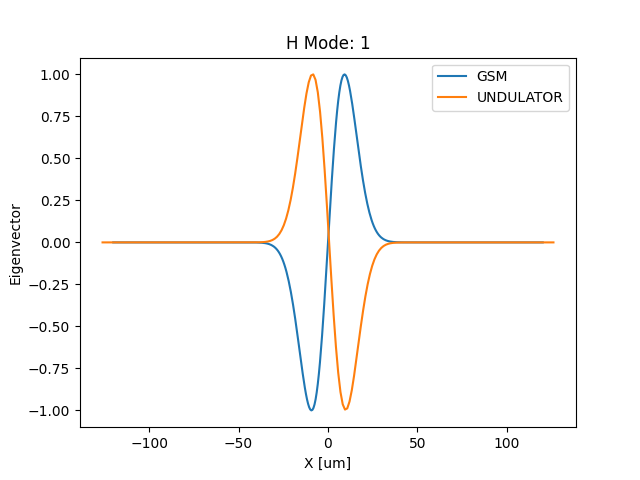
\includegraphics[width=0.49\textwidth]{figures/comparison_H_eigenvector1.png}
    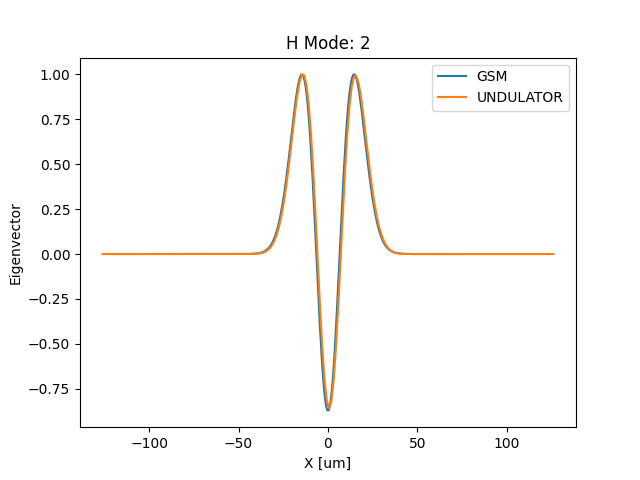
\includegraphics[width=0.49\textwidth]{figures/comparison_H_eigenvector2.png}
    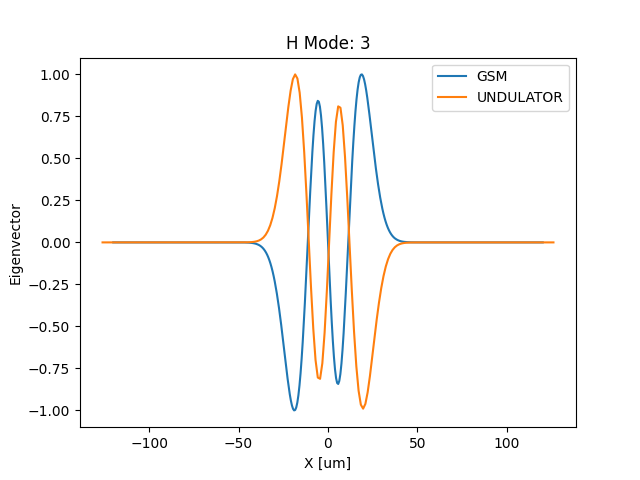
\includegraphics[width=0.49\textwidth]{figures/comparison_H_eigenvector3.png}
        
    \caption{Comparison of the approximated (GSM) and exact (1D WOFRY) coherent mode decomposition  for the Horizontal direction of a U20 undulator of length \SI{2}{\meter},  set to resonance at 10 keV photon. energy. The plot show the Cross Spectral Deisity, Spectral Density, and four first modes. The Coherence Fraction is 0.088}
    \label{fig:GSMvsUND-H}
\end{figure}


\begin{figure}
    \centering
    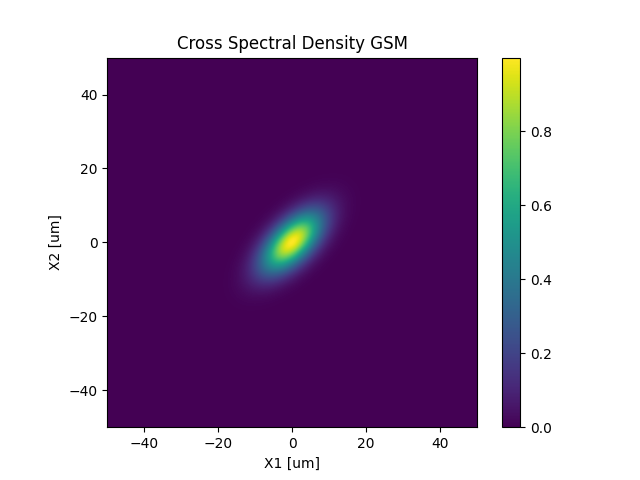
\includegraphics[width=0.49\textwidth]{figures/comparison_V_CSD_GSM.png}
    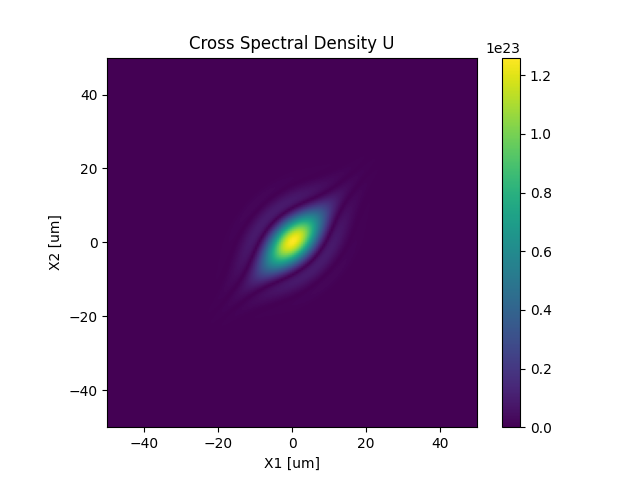
\includegraphics[width=0.49\textwidth]{figures/comparison_V_CSD_U.png}
    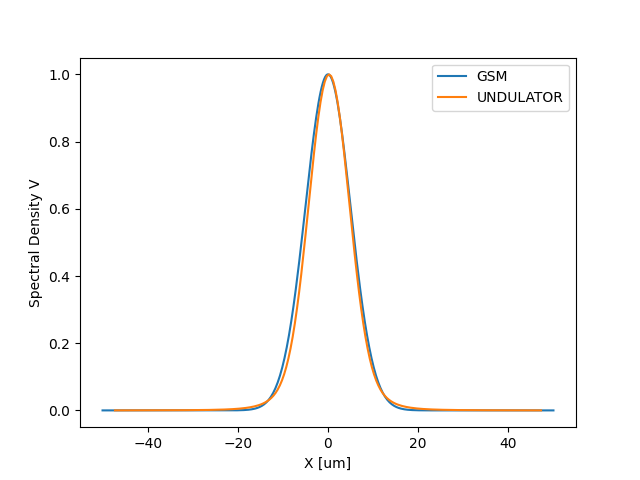
\includegraphics[width=0.59\textwidth]{figures/comparison_V_SD.png}
    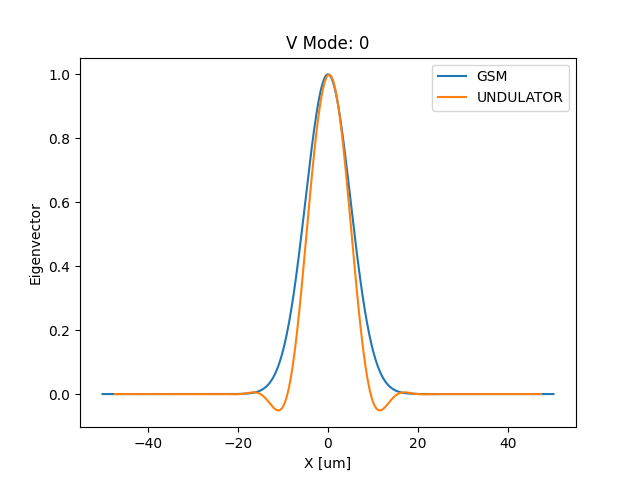
\includegraphics[width=0.49\textwidth]{figures/comparison_V_eigenvector0.png}
    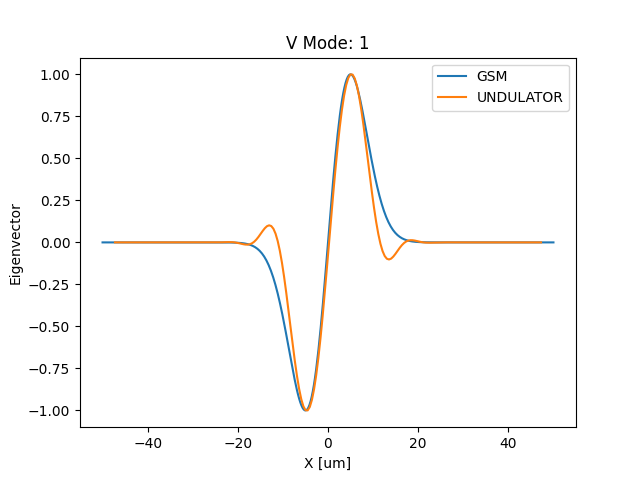
\includegraphics[width=0.49\textwidth]{figures/comparison_V_eigenvector1.png}
    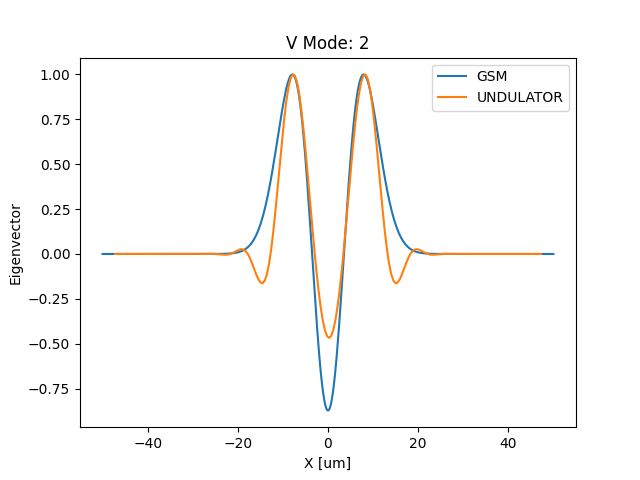
\includegraphics[width=0.49\textwidth]{figures/comparison_V_eigenvector2.png}
    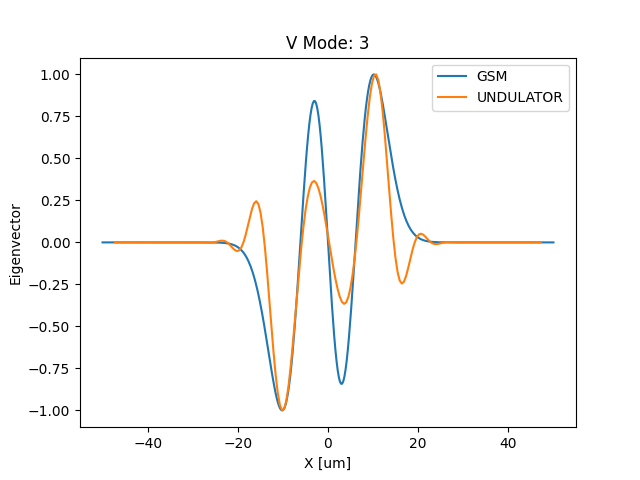
\includegraphics[width=0.49\textwidth]{figures/comparison_V_eigenvector3.png}
        
    \caption{The same as Fig.~\ref{fig:GSMvsUND-H} but for the vertical direction. The Coherence Fraction is 0.665}
    \label{fig:GSMvsUND-V}
\end{figure}



Next step is the analysis of the separability in horizontal and vertical. In Fig.~\ref{fig:GSMvsCOMSYL} we compare the coherent fraction calculated with COMSYL \cite{comsyl} and approximated by GSM (as shown in Appendix~\ref{sec:appendixA}). It shows that the GSM approximated well an undulator only for the fist modes. The Coherent Fraction (first mode) matches very well. This is due to the fact that the GSM approximation to the undulator is built matching the CF. The occupancy of higher modes differ: the first 50 GSM modes GSM to contain more than 99\% of the spectral density, but XX are needed for the numerical coherent mode decomposition with COMSYL. This means significative errors in the eigenvalues when using GSM. 

\todo{Compare COMSYL with H+V combination of WOFRY1D modes}


\begin{figure}
    \centering
    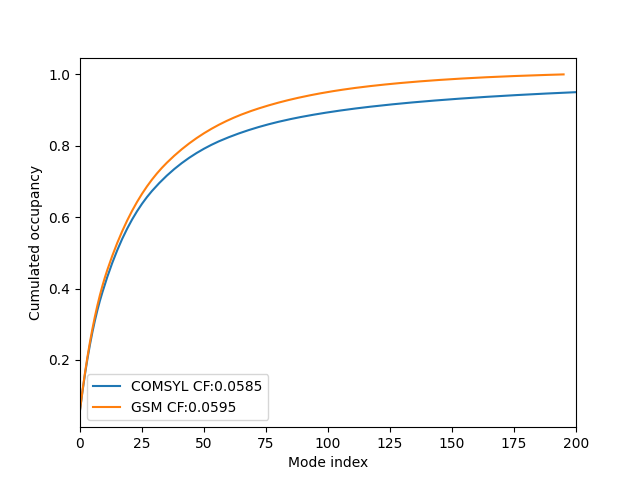
\includegraphics[width=0.95\textwidth]{figures/FigureGSMvsCOMSYL.png}
    \caption{Comparison of the approximated (GSM) and exact (COMSYL) cumulated occupation of the coherent modes for an undulator U20, of length \SI{2}{\meter}, and set to resonance at 10 keV photon. energy.}
    \label{fig:GSMvsCOMSYL}
\end{figure}

% -----------------------------------------------------------------
% -----------------------------------------------------------------
\section{Testing the effect of a slit in the GSM}
\label{appendix:slit}

In many cases the use of the GSM supposes that during propagation over the beamline elements the beam keeps its Gaussian Shell-model nature. This is true for propagation in free space, and probably true for focusing with ideal lenses. But, in the case of slits that crop the beam, it is difficult to believe that the beam is still Gaussian. Moreover, the new beam parameters $\sigma_{I'}$ and $\sigma_{\xi'}$ are obtained supposing the slit has a width $\sigma_s$, applying
\begin{equation}
    \frac{1}{\sigma_{I'}^2} = 
    \frac{1}{\sigma_{I}^2} +
    \frac{1}{\sigma_{s}^2},
\end{equation}
and
\begin{equation}
    \sigma_{\xi'} = \sigma_{\xi} 
\end{equation}

However, there are several recipes for the relation between $\sigma_s$ and the slit aperture $A$: $\sigma_s=A/4.1$, $\sigma_s=A/2.355$ and $\sigma_s=A/\sqrt{12}$.

We have calculated the case of a Gaussian beam that is cropped by a slit. The exact calculation is compared with the GSM results using the different recipes. We have used $\sigma_x$~= \SI{30}{\micro\meter} (like for the H EBS source) and three possible values of $\beta$: quite incoherent ($\beta=0.02$), medium coherence ($\beta=0.09$) and quite coherent ($\beta=1.15$). The results are in Fig.~\ref{fig:GSMslit} where the CF is compared for the exact calculation and the GSM approximation. We remind that the CF for the GSM is $CF = 1 - q$, with $q$ given in equation~\ref{q}.
The source has been created using the GSM model with a sufficient number of modes to include more that 99\% of the spectral density. Each mode is cropped by the slit placed at the source position. The Cross Spectral Density $W$ is calculated in the usual way 
\begin{equation}
    W(x_1,x_2) = \sum \lambda_i \Phi^*(x_1) \Phi(x_2),     
\end{equation}
with $\lambda_i$ the eigenvalues of the source and $\Phi(x_{1,2})$ are the eigenvectors of the source cropped by the slit. After re-diagonalizing $W$, the new eigenvalues $\lambda_i'$ permit to calculate the exact CF: 
\begin{equation}
    CF = \frac{\lambda_0'}{\sum \lambda_i'}
\end{equation}

The results in Fig.~\ref{fig:GSMslit} show two important things:
i) the GSM model usually overestimates CF in particular for high coherence ($\beta=1.15$), where there are important discrepancies between GSM and the exact calculation.
ii) For low coherence the GSM may work, in particular when using the aperture $\sigma_s=A/2.355$, i.e., matching the Gaussian FWHM with the total aperture.

\begin{figure}
    \centering
    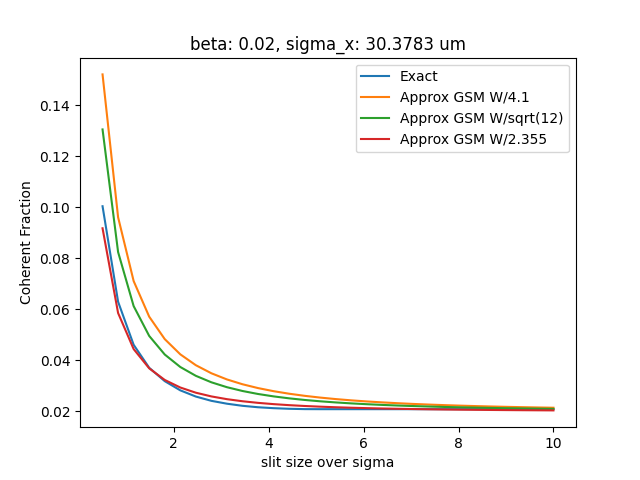
\includegraphics[width=0.95\textwidth]{figures/Figure_1a.png}
    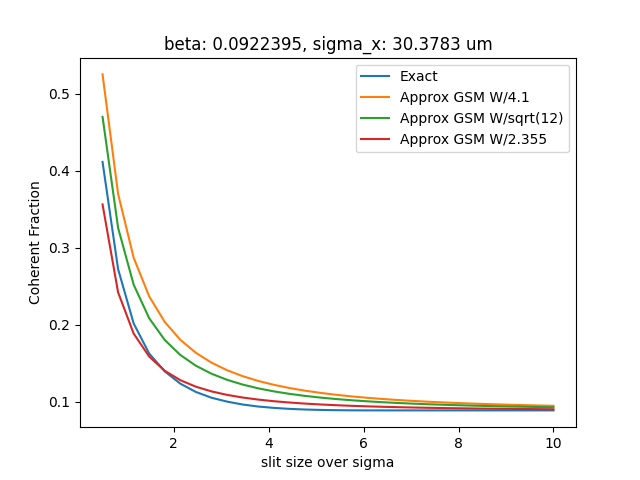
\includegraphics[width=0.95\textwidth]{figures/Figure_1b.png}
    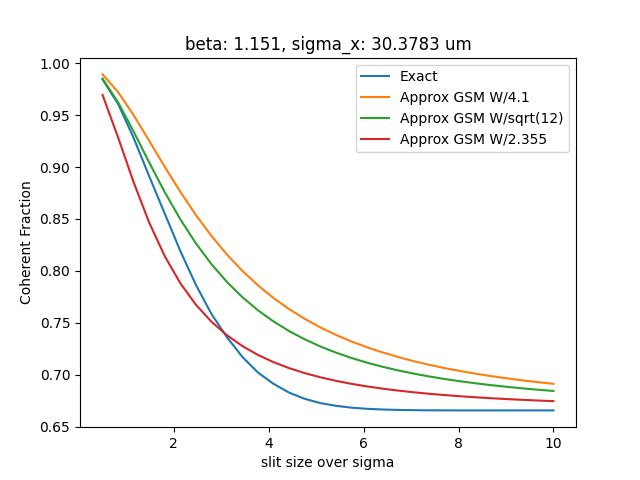
\includegraphics[width=0.95\textwidth]{figures/Figure_1c.png}
    \caption{Calculation of the coherence fraction f a Gaussian beam cropped by a slit. The exact numerical laculation (blue line) is compared with the approzimations that the beam is still described by a GSM with three possible ways to calculate the slit ``Gaussianized" $\sigma_s$ (see text). }
    \label{fig:GSMslit}
\end{figure}


% \bibliographystyle{agsm}
\bibliographystyle{vancouver}

\bibliography{iucr} % loads iucr.bib
% \referencelist{iucr}

\end{document}
